\documentclass[doc]{apa6}
\usepackage{lmodern}
\usepackage{amssymb,amsmath}
\usepackage{ifxetex,ifluatex}
\usepackage{fixltx2e} % provides \textsubscript
\ifnum 0\ifxetex 1\fi\ifluatex 1\fi=0 % if pdftex
  \usepackage[T1]{fontenc}
  \usepackage[utf8]{inputenc}
\else % if luatex or xelatex
  \ifxetex
    \usepackage{mathspec}
  \else
    \usepackage{fontspec}
  \fi
  \defaultfontfeatures{Ligatures=TeX,Scale=MatchLowercase}
\fi
% use upquote if available, for straight quotes in verbatim environments
\IfFileExists{upquote.sty}{\usepackage{upquote}}{}
% use microtype if available
\IfFileExists{microtype.sty}{%
\usepackage{microtype}
\UseMicrotypeSet[protrusion]{basicmath} % disable protrusion for tt fonts
}{}
\usepackage{hyperref}
\hypersetup{unicode=true,
            pdftitle={Working with list-columns in data.table: Proposal for rstudio::conf(2020)},
            pdfauthor={Tyson S. Barrett},
            pdfkeywords={rstudio::conf, data.table, tidyr, list-columns},
            pdfborder={0 0 0},
            breaklinks=true}
\urlstyle{same}  % don't use monospace font for urls
\usepackage{color}
\usepackage{fancyvrb}
\newcommand{\VerbBar}{|}
\newcommand{\VERB}{\Verb[commandchars=\\\{\}]}
\DefineVerbatimEnvironment{Highlighting}{Verbatim}{commandchars=\\\{\}}
% Add ',fontsize=\small' for more characters per line
\usepackage{framed}
\definecolor{shadecolor}{RGB}{248,248,248}
\newenvironment{Shaded}{\begin{snugshade}}{\end{snugshade}}
\newcommand{\AlertTok}[1]{\textcolor[rgb]{0.94,0.16,0.16}{#1}}
\newcommand{\AnnotationTok}[1]{\textcolor[rgb]{0.56,0.35,0.01}{\textbf{\textit{#1}}}}
\newcommand{\AttributeTok}[1]{\textcolor[rgb]{0.77,0.63,0.00}{#1}}
\newcommand{\BaseNTok}[1]{\textcolor[rgb]{0.00,0.00,0.81}{#1}}
\newcommand{\BuiltInTok}[1]{#1}
\newcommand{\CharTok}[1]{\textcolor[rgb]{0.31,0.60,0.02}{#1}}
\newcommand{\CommentTok}[1]{\textcolor[rgb]{0.56,0.35,0.01}{\textit{#1}}}
\newcommand{\CommentVarTok}[1]{\textcolor[rgb]{0.56,0.35,0.01}{\textbf{\textit{#1}}}}
\newcommand{\ConstantTok}[1]{\textcolor[rgb]{0.00,0.00,0.00}{#1}}
\newcommand{\ControlFlowTok}[1]{\textcolor[rgb]{0.13,0.29,0.53}{\textbf{#1}}}
\newcommand{\DataTypeTok}[1]{\textcolor[rgb]{0.13,0.29,0.53}{#1}}
\newcommand{\DecValTok}[1]{\textcolor[rgb]{0.00,0.00,0.81}{#1}}
\newcommand{\DocumentationTok}[1]{\textcolor[rgb]{0.56,0.35,0.01}{\textbf{\textit{#1}}}}
\newcommand{\ErrorTok}[1]{\textcolor[rgb]{0.64,0.00,0.00}{\textbf{#1}}}
\newcommand{\ExtensionTok}[1]{#1}
\newcommand{\FloatTok}[1]{\textcolor[rgb]{0.00,0.00,0.81}{#1}}
\newcommand{\FunctionTok}[1]{\textcolor[rgb]{0.00,0.00,0.00}{#1}}
\newcommand{\ImportTok}[1]{#1}
\newcommand{\InformationTok}[1]{\textcolor[rgb]{0.56,0.35,0.01}{\textbf{\textit{#1}}}}
\newcommand{\KeywordTok}[1]{\textcolor[rgb]{0.13,0.29,0.53}{\textbf{#1}}}
\newcommand{\NormalTok}[1]{#1}
\newcommand{\OperatorTok}[1]{\textcolor[rgb]{0.81,0.36,0.00}{\textbf{#1}}}
\newcommand{\OtherTok}[1]{\textcolor[rgb]{0.56,0.35,0.01}{#1}}
\newcommand{\PreprocessorTok}[1]{\textcolor[rgb]{0.56,0.35,0.01}{\textit{#1}}}
\newcommand{\RegionMarkerTok}[1]{#1}
\newcommand{\SpecialCharTok}[1]{\textcolor[rgb]{0.00,0.00,0.00}{#1}}
\newcommand{\SpecialStringTok}[1]{\textcolor[rgb]{0.31,0.60,0.02}{#1}}
\newcommand{\StringTok}[1]{\textcolor[rgb]{0.31,0.60,0.02}{#1}}
\newcommand{\VariableTok}[1]{\textcolor[rgb]{0.00,0.00,0.00}{#1}}
\newcommand{\VerbatimStringTok}[1]{\textcolor[rgb]{0.31,0.60,0.02}{#1}}
\newcommand{\WarningTok}[1]{\textcolor[rgb]{0.56,0.35,0.01}{\textbf{\textit{#1}}}}
\usepackage{graphicx,grffile}
\makeatletter
\def\maxwidth{\ifdim\Gin@nat@width>\linewidth\linewidth\else\Gin@nat@width\fi}
\def\maxheight{\ifdim\Gin@nat@height>\textheight\textheight\else\Gin@nat@height\fi}
\makeatother
% Scale images if necessary, so that they will not overflow the page
% margins by default, and it is still possible to overwrite the defaults
% using explicit options in \includegraphics[width, height, ...]{}
\setkeys{Gin}{width=\maxwidth,height=\maxheight,keepaspectratio}
\IfFileExists{parskip.sty}{%
\usepackage{parskip}
}{% else
\setlength{\parindent}{0pt}
\setlength{\parskip}{6pt plus 2pt minus 1pt}
}
\setlength{\emergencystretch}{3em}  % prevent overfull lines
\providecommand{\tightlist}{%
  \setlength{\itemsep}{0pt}\setlength{\parskip}{0pt}}
\setcounter{secnumdepth}{0}
% Redefines (sub)paragraphs to behave more like sections
\ifx\paragraph\undefined\else
\let\oldparagraph\paragraph
\renewcommand{\paragraph}[1]{\oldparagraph{#1}\mbox{}}
\fi
\ifx\subparagraph\undefined\else
\let\oldsubparagraph\subparagraph
\renewcommand{\subparagraph}[1]{\oldsubparagraph{#1}\mbox{}}
\fi

%%% Use protect on footnotes to avoid problems with footnotes in titles
\let\rmarkdownfootnote\footnote%
\def\footnote{\protect\rmarkdownfootnote}


  \title{Working with list-columns in \texttt{data.table}: Proposal for \texttt{rstudio::conf(2020)}}
    \author{Tyson S. Barrett\textsuperscript{1}}
    \date{}
  
\shorttitle{List-columns in data.table}
\affiliation{
\vspace{0.5cm}
\textsuperscript{1} Utah State University}
\keywords{rstudio::conf, data.table, tidyr, list-columns}
\usepackage{csquotes}
\usepackage{upgreek}
\captionsetup{font=singlespacing,justification=justified}

\usepackage{longtable}
\usepackage{lscape}
\usepackage{multirow}
\usepackage{tabularx}
\usepackage[flushleft]{threeparttable}
\usepackage{threeparttablex}

\newenvironment{lltable}{\begin{landscape}\begin{center}\begin{ThreePartTable}}{\end{ThreePartTable}\end{center}\end{landscape}}

\makeatletter
\newcommand\LastLTentrywidth{1em}
\newlength\longtablewidth
\setlength{\longtablewidth}{1in}
\newcommand{\getlongtablewidth}{\begingroup \ifcsname LT@\roman{LT@tables}\endcsname \global\longtablewidth=0pt \renewcommand{\LT@entry}[2]{\global\advance\longtablewidth by ##2\relax\gdef\LastLTentrywidth{##2}}\@nameuse{LT@\roman{LT@tables}} \fi \endgroup}

\authornote{

Correspondence concerning this article should be addressed to Tyson S. Barrett, 2800 Old Main, Logan, UT 84322. E-mail: \href{mailto:tyson.barrett@usu.edu}{\nolinkurl{tyson.barrett@usu.edu}}}

\abstract{
The use of \emph{list-columns} in data frames and tibbles is well documented (e.g.~Bryan, 2018), providing a cognitively efficient way to organize results of complex data (e.g.~several statistical models, groupings of text, data summaries, or even graphics) with corresponding data. For example, we can store text of a verse in a list for each verse, chapter, book, and volume. This allows the text to be of variable sizes without overly complicating or adding redundancies to the structure of the data. In turn, this can reduce the difficulty to appropriately analyze the data stored in the list-column. \newline

Because of its efficiency and speed, being able to use \texttt{data.table} to work with list-columns would be beneficial in many data contexts (i.e.~to reduce memory usage in large data sets). I show how one can create list-columns in a data table using \texttt{purrr::map()} and the \texttt{by} argument in \texttt{data.table}. I further show the \texttt{tidyr::nest()} function and show a more efficient approach when using a data table. Results using \texttt{microbenchmark} and \texttt{pryr} show the speed and efficiency of using \texttt{data.table} to work with list-columns. An example walk-through is provided in the appendix herein.


}

\begin{document}
\maketitle

\hypertarget{references}{%
\section{References}\label{references}}

\begingroup
\setlength{\parindent}{-0.5in}
\setlength{\leftskip}{0.5in}

\hypertarget{refs}{}
\leavevmode\hypertarget{ref-R-papaja}{}%
Aust, F., \& Barth, M. (2018). \emph{papaja: Create APA manuscripts with R Markdown}. Retrieved from \url{https://github.com/crsh/papaja}

\leavevmode\hypertarget{ref-jenny}{}%
Bryan, J. (2018). List columns (as part of "purrr tutorial"). Retrieved from \url{https://jennybc.github.io/purrr-tutorial/ls13_list-columns.html}

\leavevmode\hypertarget{ref-R-ggbeeswarm}{}%
Clarke, E., \& Sherrill-Mix, S. (2017). \emph{Ggbeeswarm: Categorical scatter (violin point) plots}. Retrieved from \url{https://github.com/eclarke/ggbeeswarm}

\leavevmode\hypertarget{ref-R-data.table}{}%
Dowle, M., \& Srinivasan, A. (2019). \emph{Data.table: Extension of `data.frame`}. Retrieved from \url{https://CRAN.R-project.org/package=data.table}

\leavevmode\hypertarget{ref-R-scriptuRs}{}%
Heiss, A. (2019). \emph{ScriptuRs: Complete text of the lds scriptures}. Retrieved from \url{https://CRAN.R-project.org/package=scriptuRs}

\leavevmode\hypertarget{ref-R-microbenchmark}{}%
Mersmann, O. (2018). \emph{Microbenchmark: Accurate timing functions}. Retrieved from \url{https://CRAN.R-project.org/package=microbenchmark}

\leavevmode\hypertarget{ref-R-base}{}%
R Core Team. (2018). \emph{R: A language and environment for statistical computing}. Vienna, Austria: R Foundation for Statistical Computing. Retrieved from \url{https://www.R-project.org/}

\leavevmode\hypertarget{ref-R-ggplot2}{}%
Wickham, H. (2016). \emph{Ggplot2: Elegant graphics for data analysis}. Springer-Verlag New York. Retrieved from \url{https://ggplot2.tidyverse.org}

\leavevmode\hypertarget{ref-R-pryr}{}%
Wickham, H. (2018). \emph{Pryr: Tools for computing on the language}. Retrieved from \url{https://CRAN.R-project.org/package=pryr}

\leavevmode\hypertarget{ref-R-stringr}{}%
Wickham, H. (2019). \emph{Stringr: Simple, consistent wrappers for common string operations}. Retrieved from \url{https://CRAN.R-project.org/package=stringr}

\leavevmode\hypertarget{ref-R-dplyr}{}%
Wickham, H., François, R., Henry, L., \& Müller, K. (2019). \emph{Dplyr: A grammar of data manipulation}. Retrieved from \url{https://CRAN.R-project.org/package=dplyr}

\leavevmode\hypertarget{ref-R-tidyr}{}%
Wickham, H., \& Henry, L. (2019). \emph{Tidyr: Easily tidy data with 'spread()' and 'gather()' functions}. Retrieved from \url{https://CRAN.R-project.org/package=tidyr}

\endgroup

\newpage

\hypertarget{appendix}{%
\section{Appendix}\label{appendix}}

To demonstrate list-columns in \texttt{data.table}, let's start with grabbing the New Testament text from the \texttt{scriptuRs} package and make it a data table. From this data table, I filtered in just the four \enquote{gospels} and selected a few important variables.

\begin{Shaded}
\begin{Highlighting}[]
\NormalTok{nt <-}\StringTok{ }\KeywordTok{data.table}\NormalTok{(scriptuRs}\OperatorTok{::}\NormalTok{new_testament)}
\NormalTok{gospels <-}\StringTok{ }
\StringTok{  }\NormalTok{nt[book_title }\OperatorTok\StringTok{ }\KeywordTok{c}\NormalTok{(}\StringTok{"Matthew"}\NormalTok{, }\StringTok{"Mark"}\NormalTok{, }\StringTok{"Luke"}\NormalTok{, }\StringTok{"John"}\NormalTok{), }
\NormalTok{     .(book_id, chapter_number, verse_number, book_title, text)]}
\end{Highlighting}
\end{Shaded}

Because we want to work with the individual words in the verses, we need to tokenize the corpus. There are two main ways we can go about this:

\begin{enumerate}
\def\labelenumi{\arabic{enumi}.}
\tightlist
\item
  Using \texttt{purrr::map()} and then \texttt{unnest()}.
\item
  Using the \texttt{by} argument in \texttt{data.table}.
\end{enumerate}

\noindent Turns out, these produce the exact same data table.

\begin{Shaded}
\begin{Highlighting}[]
\NormalTok{gospels2 <-}\StringTok{ }
\StringTok{  }\NormalTok{gospels[, .(book_id, chapter_number, verse_number, book_title, text,}
              \DataTypeTok{tokens =}\NormalTok{ purrr}\OperatorTok{::}\KeywordTok{map}\NormalTok{(text, }\OperatorTok{~}\NormalTok{tm}\OperatorTok{::}\KeywordTok{MC_tokenizer}\NormalTok{(.x)))] }\OperatorTok\StringTok{ }
\StringTok{  }\KeywordTok{unnest}\NormalTok{()}
\NormalTok{gospels3 <-}\StringTok{ }
\StringTok{  }\NormalTok{gospels[, .(}\DataTypeTok{tokens =}\NormalTok{ tm}\OperatorTok{::}\KeywordTok{MC_tokenizer}\NormalTok{(text)), }
\NormalTok{          by =}\StringTok{ }\NormalTok{.(book_id, chapter_number, verse_number, book_title, text)]}
\KeywordTok{all.equal}\NormalTok{(gospels2, gospels3)}
\end{Highlighting}
\end{Shaded}

\begin{verbatim}
## [1] TRUE
\end{verbatim}

\noindent And both take about the same amount of memory and time to complete.

\begin{Shaded}
\begin{Highlighting}[]
\NormalTok{exp1 <-}\StringTok{ }\KeywordTok{expression}\NormalTok{(}
\NormalTok{  gospels[, .(book_id, chapter_number, verse_number, book_title, text,}
              \DataTypeTok{tokens =}\NormalTok{ purrr}\OperatorTok{::}\KeywordTok{map}\NormalTok{(text, }\OperatorTok{~}\NormalTok{tm}\OperatorTok{::}\KeywordTok{MC_tokenizer}\NormalTok{(.x)))] }\OperatorTok\StringTok{ }
\StringTok{    }\KeywordTok{unnest}\NormalTok{()}
\NormalTok{)}
\NormalTok{exp2 <-}\StringTok{ }\KeywordTok{expression}\NormalTok{(}
\NormalTok{  gospels[, .(}\DataTypeTok{tokens =}\NormalTok{ tm}\OperatorTok{::}\KeywordTok{MC_tokenizer}\NormalTok{(text)), }
          \DataTypeTok{by =}\NormalTok{ .(book_id, chapter_number, verse_number, book_title, text)]}
\NormalTok{)}
\end{Highlighting}
\end{Shaded}

\begin{verbatim}
##      kilobytes
## exp1   -10.336
## exp2    34.712
\end{verbatim}

\begin{verbatim}
## Unit: seconds
##    expr      min       lq     mean   median       uq      max neval cld
##  unnest 3.779131 3.817389 3.842819 3.832526 3.842268 3.955123    10   a
##      by 3.744560 3.768794 3.830423 3.814809 3.895425 3.929232    10   a
\end{verbatim}

\noindent As such, we'll use the \texttt{purrr::map()} approach since it gives us the intermediate data, that of \textbf{list-columns}. This time we'll use \texttt{:=} to simplify the workflow. This will modify-in-place, changing the \texttt{gospels} object without copying it.

\begin{Shaded}
\begin{Highlighting}[]
\NormalTok{gospels[, tokens }\OperatorTok{:}\ErrorTok{=}\StringTok{ }\NormalTok{purrr}\OperatorTok{::}\KeywordTok{map}\NormalTok{(text, }\OperatorTok{~}\NormalTok{tm}\OperatorTok{::}\KeywordTok{MC_tokenizer}\NormalTok{(.x))]}
\NormalTok{gospels[, .(tokens)]}
\end{Highlighting}
\end{Shaded}

\begin{verbatim}
##                                          tokens
##    1:         THE,book,of,the,generation,of,...
##    2:   Abraham,begat,Isaac,and,Isaac,begat,...
##    3:       And,Judas,begat,Phares,and,Zara,...
##    4:  And,Aram,begat,Aminadab,and,Aminadab,...
##    5:       And,Salmon,begat,Booz,of,Rachab,...
##   ---                                          
## 3775:       Peter,seeing,him,saith,to,Jesus,...
## 3776:             Jesus,saith,unto,him,If,I,...
## 3777:    Then,went,this,saying,abroad,among,...
## 3778: This,is,the,disciple,which,testifieth,...
## 3779:         And,there,are,also,many,other,...
\end{verbatim}

With this updated \texttt{gospels} data table, we can unnest it with \texttt{tidyr::unnest()}.

\begin{Shaded}
\begin{Highlighting}[]
\NormalTok{unnested_gospels <-}\StringTok{ }\KeywordTok{unnest}\NormalTok{(gospels)}
\end{Highlighting}
\end{Shaded}

\noindent We can also nest it again. If we use it raw with \texttt{tidyr::nest()}, it produces a data frame (no longer a data table).

\begin{Shaded}
\begin{Highlighting}[]
\KeywordTok{nest}\NormalTok{(unnested_gospels, tokens, }\DataTypeTok{.key =} \StringTok{"tokens"}\NormalTok{) }\OperatorTok\StringTok{ }
\StringTok{  }\KeywordTok{class}\NormalTok{()}
\end{Highlighting}
\end{Shaded}

\noindent Instead, we are going to use a custom function that uses the power of the \texttt{by} argument in \texttt{data.table} to keep the data a data table while taking advantage of the efficiency and speed of \texttt{data.table}.

\begin{Shaded}
\begin{Highlighting}[]
\NormalTok{nest_dt <-}\StringTok{ }\ControlFlowTok{function}\NormalTok{(dt, ..., }\DataTypeTok{.key =} \StringTok{"data"}\NormalTok{, }\DataTypeTok{by =} \StringTok{"id"}\NormalTok{)\{}
  \KeywordTok{stopifnot}\NormalTok{(}\KeywordTok{is.data.table}\NormalTok{(dt))}
  
\NormalTok{  j <-}\StringTok{ }\KeywordTok{substitute}\NormalTok{(}\KeywordTok{list}\NormalTok{(...))}
\NormalTok{  by <-}\StringTok{ }\KeywordTok{substitute}\NormalTok{(by)}
  
\NormalTok{  express <-}\StringTok{ }\NormalTok{dt[, }\KeywordTok{list}\NormalTok{(}\KeywordTok{eval}\NormalTok{(j)), by =}\StringTok{ }\KeywordTok{eval}\NormalTok{(by)]}
  \KeywordTok{setnames}\NormalTok{(express, }\DataTypeTok{old =} \StringTok{"V1"}\NormalTok{, }\DataTypeTok{new =}\NormalTok{ .key)}
\NormalTok{  express}
\NormalTok{\}}
\end{Highlighting}
\end{Shaded}

Since having a \texttt{data.table} may be important for our workflow, this custom function be compared with the regular \texttt{tidyr::nest()} function with the \texttt{data.table()}. Below, the \texttt{tidyr::nest()} without \texttt{data.table()} is also compared, showing that the results are not due to the addition of \texttt{data.table()}.

\begin{Shaded}
\begin{Highlighting}[]
\NormalTok{regular <-}\StringTok{ }\KeywordTok{expression}\NormalTok{(}
  \KeywordTok{nest}\NormalTok{(unnested_gospels, tokens, }\DataTypeTok{.key =} \StringTok{"tokens"}\NormalTok{)}
\NormalTok{)}
\NormalTok{regular_dt <-}\StringTok{ }\KeywordTok{expression}\NormalTok{(}
  \KeywordTok{nest}\NormalTok{(unnested_gospels, tokens, }\DataTypeTok{.key =} \StringTok{"tokens"}\NormalTok{) }\OperatorTok\StringTok{ }\KeywordTok{data.table}\NormalTok{()}
\NormalTok{)}
\NormalTok{custom <-}\StringTok{ }\KeywordTok{expression}\NormalTok{(}
  \KeywordTok{nest_dt}\NormalTok{(unnested_gospels, tokens, }\DataTypeTok{.key =} \StringTok{"tokens"}\NormalTok{, }
          \DataTypeTok{by =}\NormalTok{ .(book_id, chapter_number, verse_number, book_title, text))}
\NormalTok{)}
\end{Highlighting}
\end{Shaded}

\begin{table}[tb]
\centering
\caption{Memory change from using each nesting approach.} 
\begin{tabular}{rr}
  \hline
 & kilobytes \\ 
  \hline
regular & 64204.98 \\ 
  regular\_dt & 63962.05 \\ 
  custom & 53.62 \\ 
   \hline
\end{tabular}
\end{table}

Results of these comparisons for this data set show that using the \texttt{data.table} approach is far more efficient (\(\approx\) 64,000 kB for \texttt{tidyr::nest()} vs.~54 kB for \texttt{data.table} with \texttt{by} argument; see Table 1) and far faster (see Figure 1), yet produces the list-columns just as is desired. Beyond the comparisons, however, this example shows that the benefits of list-columns can be found in data tables.

\begin{figure}[htb]
  \centering
  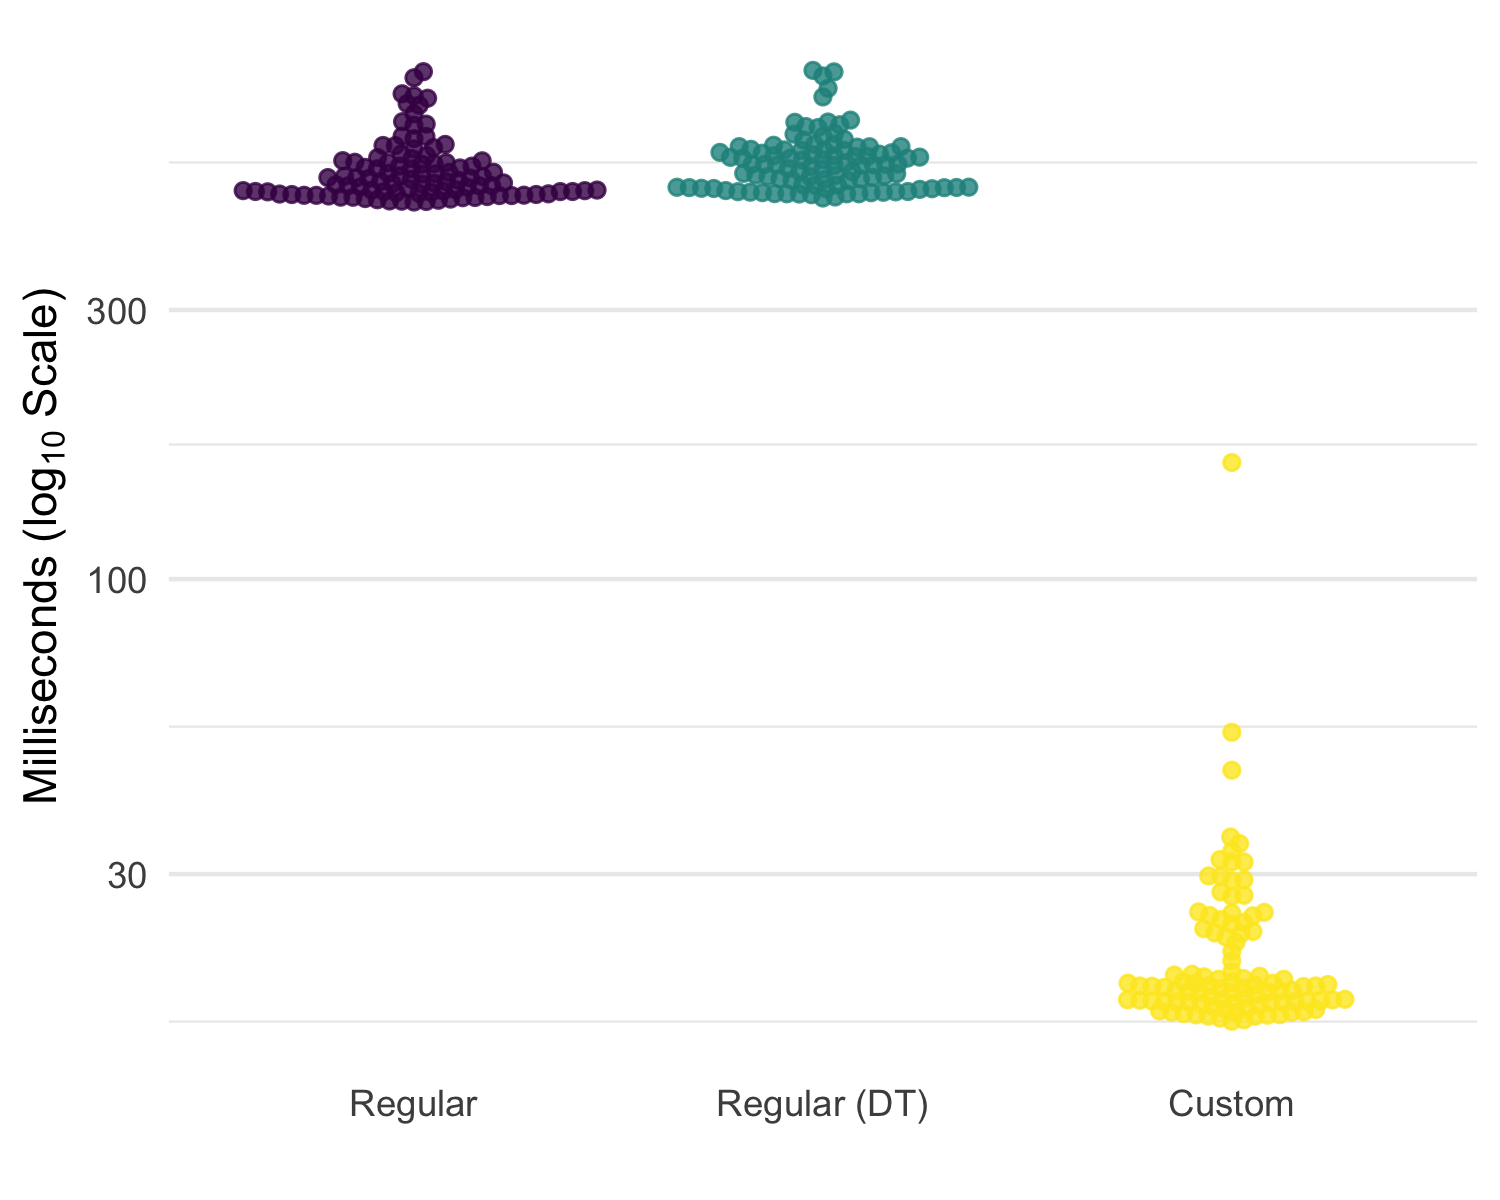
\includegraphics[width=0.7\textwidth]{timings.png}
  \caption{Speed comparisons for each nesting approach.}
\end{figure}


\end{document}
